\documentclass[border=10pt]{standalone}

\usepackage{tikz}
\usepackage{tikzsymbols}
\usetikzlibrary{calc,patterns,shapes.geometric}

\def\centerarc[#1](#2)(#3:#4:#5){\draw[#1] ($(#2)+({#5*cos(#3)},{#5*sin(#3)})$) arc (#3:#4:#5);}

\begin{document}
	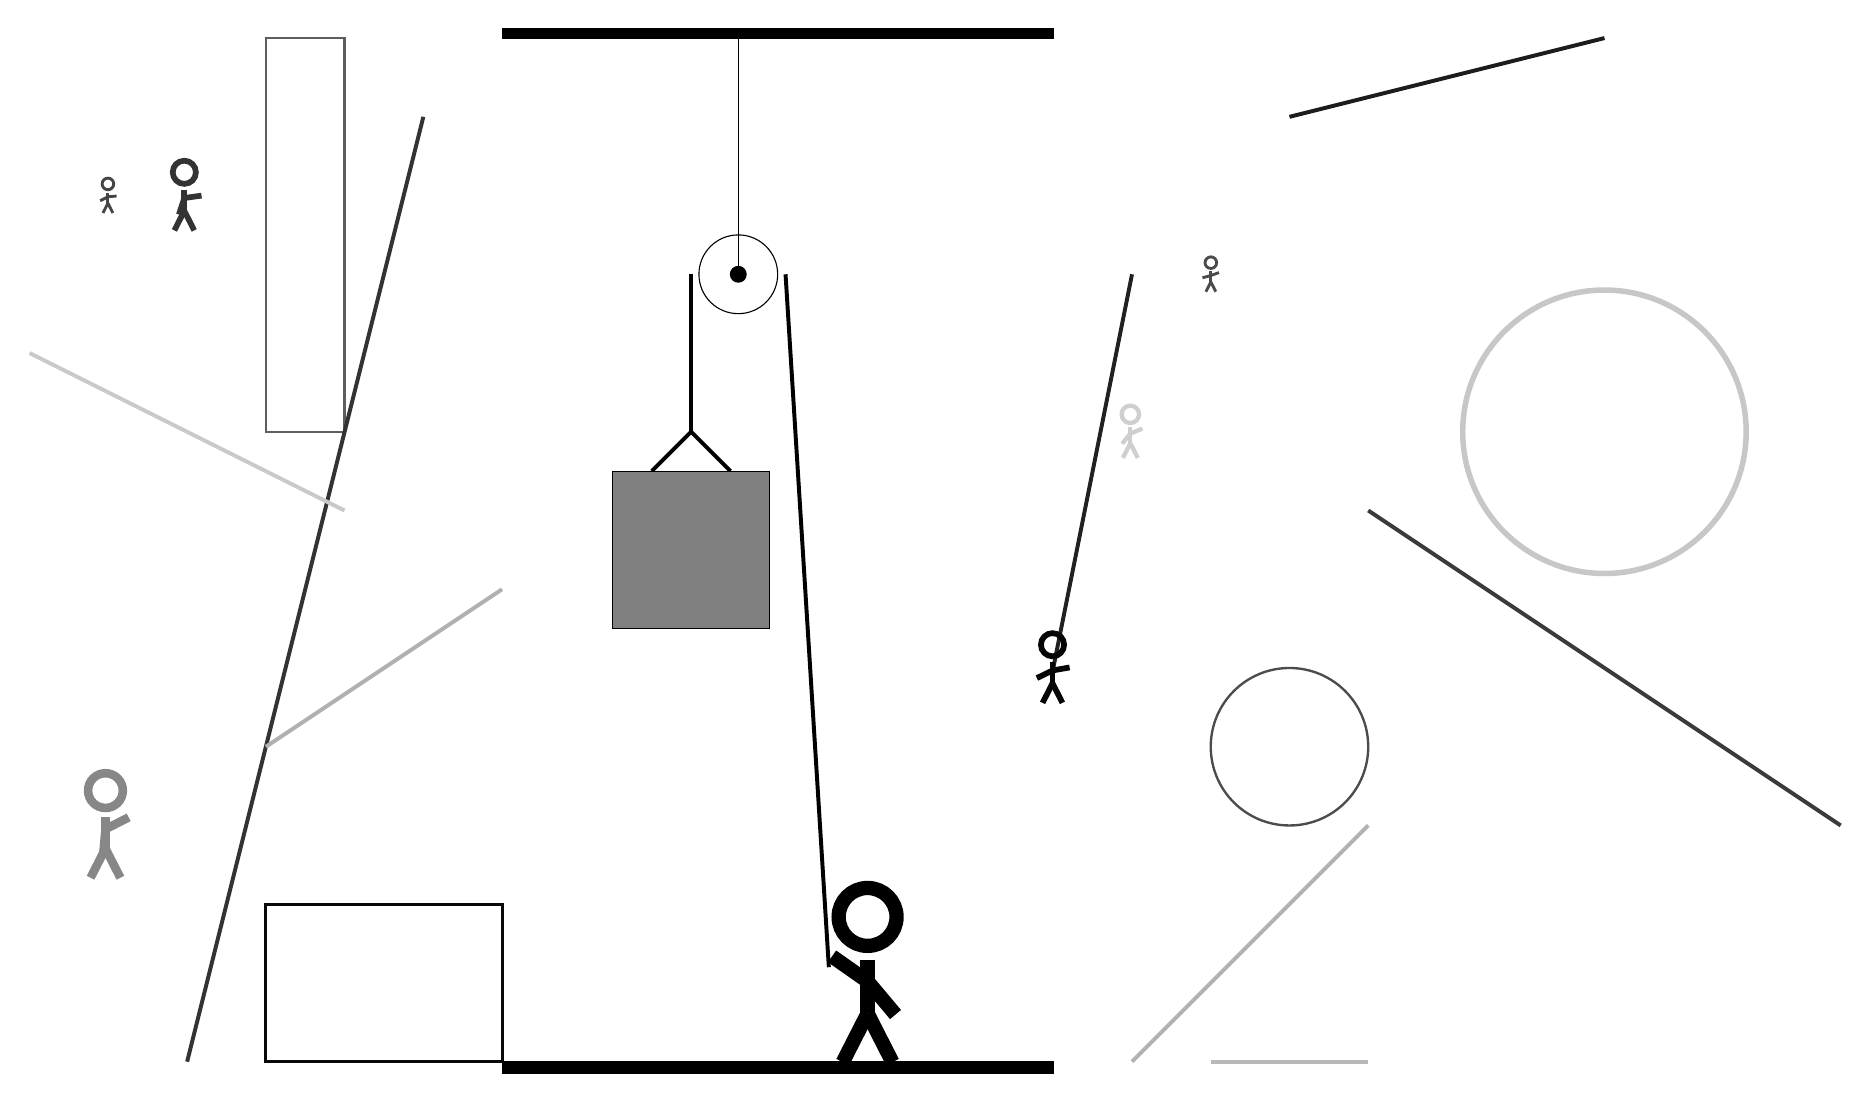
\begin{tikzpicture}
		%%%%% START %%%%%
		
		\draw[fill=black] (-2, 10) rectangle (5, 10.125);
		
		\draw (1, 7) circle (0.5);
		\draw[fill=black] (1, 7) circle (0.1);
		\draw (1, 10) -- (1, 7);
		
		\draw[line width=0.5mm] (-0.1, 4.5) -- (0.4, 5.0) -- (0.9, 4.5);
		\draw[fill=black!50] (-0.6, 4.5) rectangle (1.4, 2.5);
		
		\draw[line width=0.5mm] (0.4, 7) -- (0.4, 5.0);
		\centerarc[line width=0.5mm](1, 7)(0:180:0.6);
		\draw[line width=0.5mm](1.6, 7) -- (2.15, -1.8);
		
		\draw[line width=0.5mm, color=black!89](8, 9) -- (12, 10);
		
		\draw[line width=0.5mm, color=black!87](5, 2) -- (6, 7);
		\draw [line width=0.3mm, color=black!70](8, 1) circle (1.0);
		\node[line width=0.2mm, color=black!80] at (-6, 8) {\Strichmaxerl[4][72][8]};
		\node[line width=0.3mm, color=black!71] at (7, 7) {\Strichmaxerl[2][15][20]};
		
		\draw[line width=0.3mm, color=black!63] (-4, 5) rectangle (-5, 10);
		
		\node[line width=0.4mm, color=black!47] at (-7, 0) {\Strichmaxerl[6][85][27]};
		\node[line width=0.6mm, color=black!19] at (6, 5) {\Strichmaxerl[3][51][23]};
		\draw[line width=0.5mm, color=black!80](-6, -3) -- (-3, 9);
		\draw[line width=0.5mm, color=black!30](6, -3) -- (9, 0);
		\node[line width=0.3mm, color=black!98] at (5, 2) {\Strichmaxerl[4][26][10]};
		\draw[line width=0.5mm, color=black!77](9, 4) -- (15, 0);
		\draw[line width=0.5mm, color=black!28](9, -3) -- (7, -3);
		
		\draw [line width=0.7mm, color=black!22](12, 5) circle (1.8);
		\draw[line width=0.5mm, color=black!31](-5, 1) -- (-2, 3);
		\draw[line width=0.4mm, color=black!97] (-2, -3) rectangle (-5, -1);
		\draw[line width=0.5mm, color=black!21](-4, 4) -- (-8, 6);
		
		\node[line width=0.6mm, color=black!73] at (-7, 8) {\Strichmaxerl[2][27][5]};
		
		\node at (2.6, -1.9) {\Strichmaxerl[10][-35][-50]};
		
		\draw[fill=black] (-2, -3) rectangle (5, -3.15);
		
		%%%%% END %%%%%
	\end{tikzpicture}
\end{document}